\documentclass[11pt, a4paper]{article}

\usepackage{amsmath}
\usepackage{amsfonts} %Matheschriften
\usepackage{amssymb} %Mathesymbole
%\usepackage{mathptmx} % Einstellung für Schriften und Sonderzeichen in mathematischen Umgebungen
                        % ändert SChriftfont
\usepackage{wasysym} % Stellt diverse Sonderzeichen bereit
\usepackage{siunitx}
\usepackage{float}
\usepackage{microtype}
\usepackage{graphicx}
\usepackage{hyperref}
\usepackage{xcolor}
\usepackage[section]{placeins}
% allows for temporary adjustment of side margins
\usepackage{changepage}
\usepackage{rotating}
\usepackage{physics}

\usepackage[ngerman]{babel}
\addto\captionsngerman{%
 \renewcommand{\abstractname}{Einleitung}}


\title{Versuch 3: Beugung und Brechung}
\author{Team 4-11: Jascha Fricker, Benedict Brouwer}

\begin{document}
    \maketitle

    \tableofcontents

    \newpage

    \section{Theorie}
    \FloatBarrier
    In diesem Versuch wurde mit einem Einfachspalt, einem Gitter und einem Prisma Phänomene der Beugung und Brechung untersucht. 

    \subsection{Beugung am Einfachspalt}
    Bei bestrahlung eines Einfachspalts (mit Spaltbreite $d$) mit kohärentem Licht der Wellenlänge $\lambda$ entsteht auf dem Schirm mit Abstand $l$ ein Beugungsbild bestehend aus Minima und Maxima mit Abstand $s$ zum Maxima nullter Ordnung. Dessen Position kann mit folgenden Fromeln berechnet werden:
    \begin{align}
        \frac{n * \lambda}{d} = sin{\alpha} \approx \tan{\alpha} = \frac{s_{Minima}}{l} \label{eq:einfachspalt} \\
        \frac{(n + \frac{1}{2})* \lambda}{d} = sin{\alpha} \approx \tan{\alpha} = \frac{s_{Maxima}}{l} 
    \end{align}
    \subsection{Beugung am Gitter}
    Wird ein Gitter mit Gitterkonstante $a$ bestrahlt so entsteht auf dem Schirm ein charakteristisches Beugungsbilt mit Hauptmaxima n-ter Ordnung mit Entfernung $s$ zum Mittelpunkt. Deren Position Kann Berechnet werden mit:
    \begin{align}
        \frac{n * \lambda}{a} = sin{\alpha} \approx \tan{\alpha} = \frac{s_{Maxima}}{l} \label{eq:Gitter} \\
    \end{align}

    \subsection{Brechung am Prisma}

    \paragraph{Brechunsindex}
    Der Brechungsindex $n$ kann aus dem minimalen Ablenkungswinkel $\delta_{min}$ und dem Winkel $e$ des Prismas mit der Formel
    \begin{align}
        n = \frac{\sin\left(\frac{d_{min} + e}{2}\right)}{\sin\left(\frac{e}{2}\right)} \label{eq:brechungsindex}
    \end{align}
    berechnet werden.
    
    \section{Ergebnisse}
    \subsection{Einfachspalt}
    In diesem Versuchsteil wurde mit einem Laser der Wellenlänge $\lambda = 532(1)\si{\nano\meter}$ ein Einfachspalt bestrahlt und dessen Beugungsbild untersucht.
    Dazu wurde bei drei unterschiedlichen Schirmabständen der Abstand der Minima der Jeweiligen Ordnung zueinander gemessen. Bei der Auswertung wurde die Kleinwinkelnäherung angewerndet, da im Extremalfall $\arctan(\frac{s}{l}) = 1,1457°$ und $\arcsin(\frac{s}{l}) = 1,1459°$
    was einer Abweichung von $0,017\%$ entspricht. Die Messergebnisse wurden in Graph \ref{fig:einzelspalt} geplottet und mit einer Ausgleichsgerade $a \cdot x + b$ mit den Parametern $a = 3,64(13) \cdot 10^{-3}$ und $b= -1,05 \cdot 10^{-4}$ gefittet.
    Mit disen Parameter lässt sich aus Formel \ref{eq:einfachspalt} und mithilfe der gaußschen Fehlerfortpflanzung die Spaltbreite berechnen zu $d= 146(5) \cdot 10^{-3}$. Die Fehlerbalken wurden mit dem Analogenfehler eines Metermaßes und Fehlerfortpflanzung berechent.
    


    \begin{figure}
        \centering
        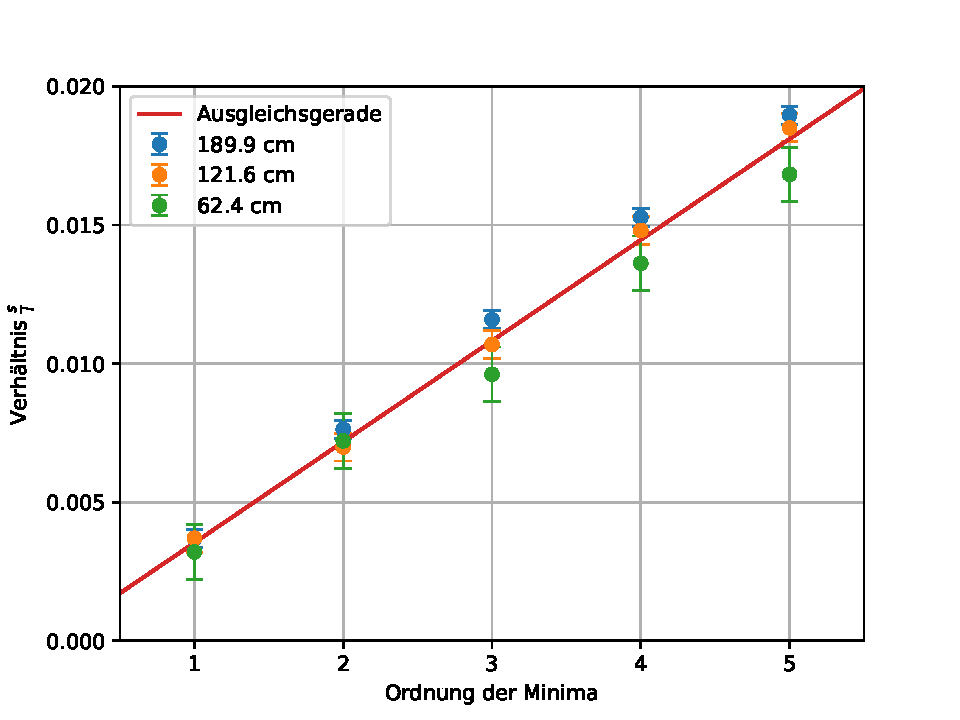
\includegraphics[width=0.8\textwidth]{./plots/einzelspalt.pdf}
        \caption{Messergebnisse des Einzelspalts}
        \label{fig:einzelspalt}
    \end{figure}
    \subsection{Berechnung der Wellenlängen einer Hg Lampe}
    Um die charakteristischen Wellenlängen einer Quksilberdampf-Lampe zu bestimmen wird in diesem Versuchsteil deren Licht auf ein Gitter mit einer Gitterkonstante von $a=10.00(02)\cdot \si{\micro\metre}$ gerichtet.
    Anschließend wurde bei drei unterschiedlichen Abständen der Abstand der Maxima gleicher Ordnung zueinander gemessen für drei der Charakteristischen Wellenlängen. Hirbei kann nicht von der Kleinwinkelnäherung gebrauch gemacht werden, da im Extremalfall $\arctan(\frac{s}{l}) = 14.574°$ und $\arcsin(\frac{s}{l}) = 15,070°$
    was einer Abweichung von $2,14\%$ entspricht. Daher wurde in der Auswertung $\sin(\arctan(\frac{s}{l}))$ gegen die Ordnung der Maxima für die Drei Wellenlängen wie in den Graphen \ref{fig:GitterBLAU}, \ref{fig:GitterGRÜN} und \ref{fig:GitterROT} zu sehen aufgetragen.
    Dabei fällt auf, das die Messwerte des Abstandes $26,15 \si{\centi\metre}$ eine hohe ungenauhigkeit aufweisen, was vermutlich an dem kleineren Abstand der Maxima bei dieser Länge liegt.
    Mit den Parametern der Ausgleichsgeraden kann nun mit Formel \ref{eq:Gitter} kann nun für jede Farbe die Wellenlänge berechnet werden. Die Ergebnisse sind in Tabelle \ref{tab:Gitter} mit den Literaturwerten verglichen. Die Ergebnisse liegen nahe an den Literaturwerten allerdings mit einem großen Fehler von bis zu 40 nm.
    Dieser lässt sich mit dem großen Fehler des Fits erklären aufgrund der großen ungenauhigkeit bei Abstand a =  $26,15 \si{\centi\metre}$. Zur Fehler berechung fließen die analogen Fehler in den Fehler des Fits mit ein welcher dann mit gaußscher Fehlerfortpflanzung mit dem Fehler der Gitterkonstante kombiniert wird.

    \begin{figure}
        \centering
        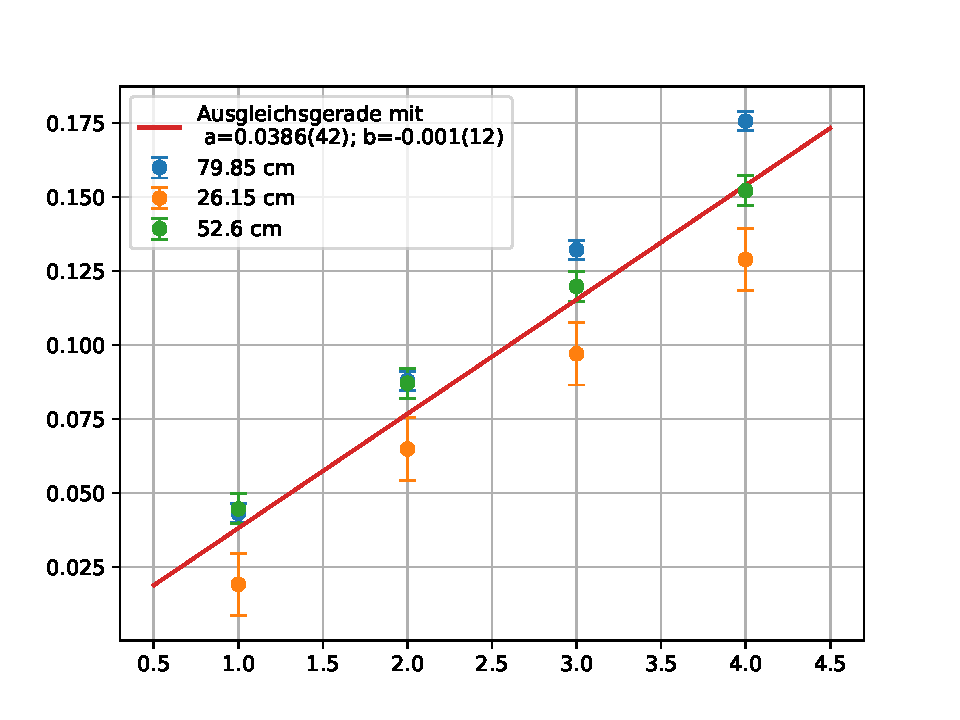
\includegraphics[width=0.8\textwidth]{./plots/Gitter_Blau.pdf}
        \caption{Messergebnisse am Gitter der blauen Wellenlänge}
        \label{fig:GitterBLAU}
    \end{figure}
    \begin{figure}
        \centering
        \includegraphics[width=0.8\textwidth]{./plots/Gitter_Grün.pdf}
        \caption{Messergebnisse am Gitter der grünen Wellenlänge}
        \label{fig:GitterGRÜN}
    \end{figure}
    \begin{figure}
        \centering
        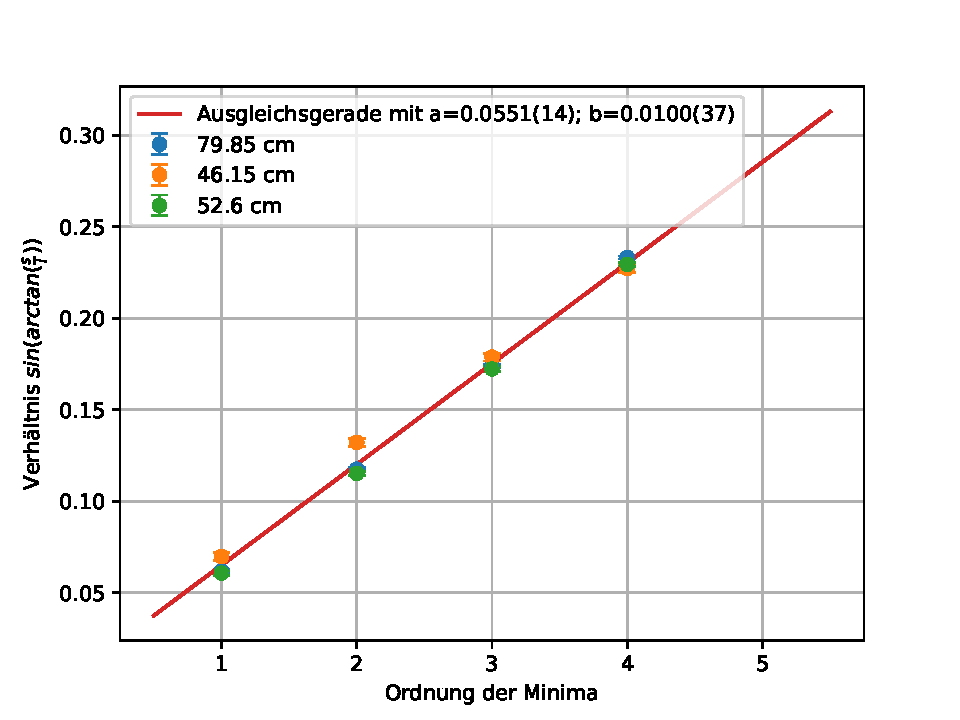
\includegraphics[width=0.8\textwidth]{./plots/Gitter_Rot.pdf}
        \caption{Messergebnisse am Gitter der roten Wellenlänge}
        \label{fig:GitterRot}
    \end{figure}

    \begin{table}
        \centering
        \begin{tabular}{c|c|c|c}
            
            Farbe & Steigung der Ausgleichsgeraden & Wellenlänge $\lambda in \si{\nano\metre}$  & Literaturwert  $\lambda_{lit} in \si{\nano\metre}$\\ \hline
            Grün & 0,0549(33) & 549(33) & 546 \\ \hline
            Blau &  0,0386(42) & 390(40) & 405 \\ \hline
            Rot & 0,0574(39) & 570(40) &577 bzw. 579  \\\hline

        \end{tabular}
        \caption{Ergebnisse der Hg-Lampe}
        \label{tab:Gitter}
    \end{table}

    \subsection{Prisma}
    \paragraph{Prismenwinkel}
    Der Prismenwinkel $e$ kann durch die Mesung der beiden Reflektionswinkel $\phi = 124,10(2)^{\circ}$ und $\theta = 4,10(2)^{\circ}$ bei Beleuchtung genau auf die Kante des Prismas bestimmt werden. Es gilt
    \begin{align}
        e = \frac{\phi - \theta}{2} = 60,000(14)^{\circ} \label{eq:prisma} \ .
    \end{align}
    Als Fehler wurde eine anaoge Ableseungenauigkeit von $0,1^{\circ}$ angenommen.

    \paragraph{Brechungsindex}
    Mit Formel \ref{eq:brechungsindex} kann der Brechungsindex des Prismenmaterials in Abhängigkeit von der Wellenlänge berechnet werden. Die berechneten Werte und die gemessen Werte sind in Tabelle \ref{tab:prisma} zusammengefasst. Die Wellenlängenaghängigkeit kann durch eine Gerade genähert werden. Die und der Fit sind in Abbildung \ref{fig:prisma} gezeigt. Die gefittete Kurve stimmt nicht mit den Unsicherheiten überein. Das kann aber daran liegen, dass für die Winkelunsicherheit nur die digitale Unsicherheit von $0,1^{\circ}$ berücksichtigt wurde, also $0,04^{\circ}$ für die Differenz von zwei Messwerten.

    % n =  0.647+/-0.017  bei  578.0+/-1.0 nm winkel =  48.20+/-0.04 °
    % n =  0.788+/-0.014  bei  546.07+/-0 nm winkel =  48.60+/-0.04 °
    % n =  0.987+/-0.005  bei  435.83+/-0 nm winkel =  50.40+/-0.04 °


    \begin{table}[h]
        \centering
        \begin{tabular}{c|c|c}
            Wellenlänge $\lambda in \si{\nano\metre}$ \cite{Wiki} & Winkel & Brechungsindex $n$ \\ \hline
            $577/579 \si{\nano\meter}$ & $48,20(04)^{\circ}$ & $0,647(017)$ \\ \hline
            $546,07 \si{\nano\meter}$ & $48,60(04)^{\circ}$ & $0,788(014)$ \\ \hline
            $435,83 \si{\nano\meter}$ & $50,40(04)^{\circ}$ & $0,987(005)$ \\ \hline
        \end{tabular}
        \caption{Ergebnisse der Prisma Messung}
        \label{tab:prisma}     
    \end{table}

    \begin{figure}
        \centering
        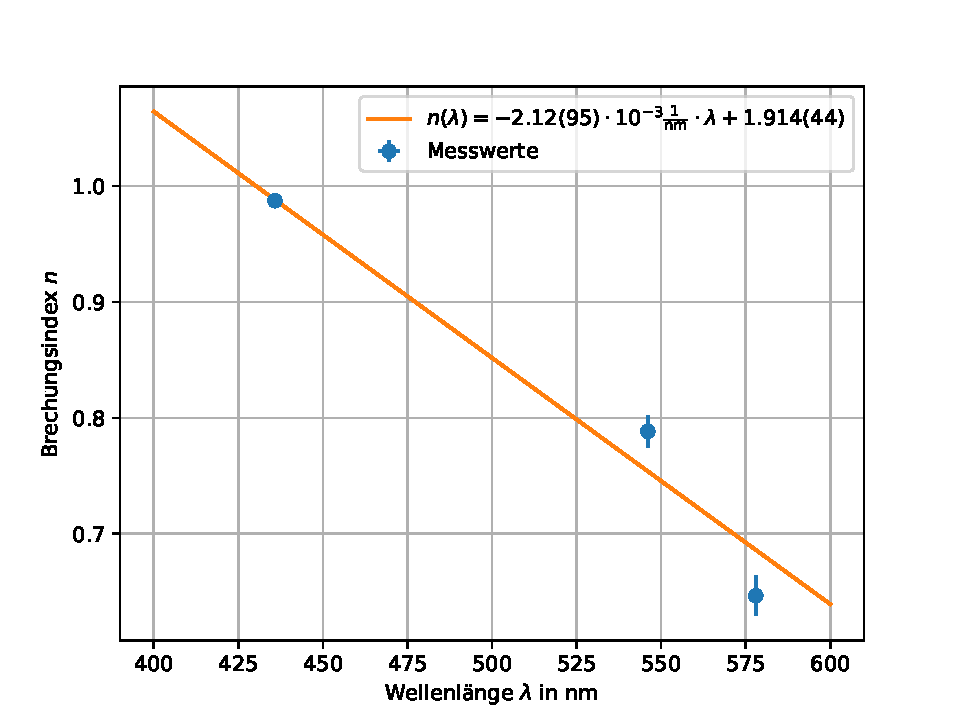
\includegraphics[width=0.8\textwidth]{plots/prism1.pdf}
        \caption{Brechungsindex des Prismas}
        \label{fig:prisma}
    \end{figure}

    \paragraph{Energiesparlampe}
    Aus den gemessenen Winkeln lassen sich mit vorher berechneten gefitteten Gerade aus den Winkeln die Wellenlänen der Linien berechnen. Die Ergebnisse sind in Tabelle \ref{tab:energiesparlampe} zusammengefasst. Die Wellenlängen passen zu den beobachteten Farben von grün und rot. Dadurch dass es viele verschiede Bauarten von Energiesparlampen gibt, konnten keine eindeutigen Literaturwert gefunden werden, mit dehnen verglichen werden kann.

    % Energie =  48.7 °  bei  515.4+/-2.5 nm n =  0.819+/-0.005
    % Energie =  47.5 °  bei  740.8+/-3.4 nm n =  0.340+/-0.007

    \begin{table}[h]
        \centering
        \begin{tabular}{c|c|c}
            Wellenlänge $\lambda in \si{\nano\metre}$ & Winkel & Brechungsindex $n$ \\ \hline
            $515,4 \si{\nano\meter}$ & $48,7^{\circ}$ & $0,819$ \\ \hline
            $740,8 \si{\nano\meter}$ & $47,5^{\circ}$ & $0,340$ \\ \hline
        \end{tabular}
        \caption{Ergebnisse der Energiesparlampe}
        \label{tab:energiesparlampe}
    \end{table}

    \bibliographystyle{plain}
    \bibliography{literature}

\end{document}